\chapter{RESULTS AND DISCUSSION}
\section{Data}
%The data will be generated with the common technique of rejection sampling,
%where n high dimensional seeds are chosen at random, samples will be taken
%at random from a uniform distribution, if the sample falls with in radius r of
%any seed it is accepted, if it does not, single random number is drawn, if that
%number is \(<\) 0.05\% the sample is accepted as noise, else the sample is rejected.
The training data will be generated using a Gaussian cluster generator as
described by \cite{handl}. To generate the data we have to decide how many
clusters to create and how many dimmension to use.  In order to set these
parameters appropiatly we will first explore how the internal variance
responds to adjustments in their value.

To accomplish this twenty test data sets are genorated and used to train both
the rook and sphereical SOMs. As shown in tables \ref{ivtable1} and
\ref{ivtable2} both topologies seem to respond similarly. The internal
variance of the SOM increases as we add dimmeniosn and decreases as we add
clusters. Based on these tables, it was decided that five dimmensions and ten
clusters was a reasonable choice. Five dimmeniosn is easier to work with than
large numbers and should yield more information than two dimmensions. 

With these paramaters choosen ten data sets are generated and used to train
SOMs for each topology.  After running ten simulations for both the rook and
sphereical toplogies we find that the mean internal variance seems to remain
fairly stable, this suggests that we can combine these to compare across
topologies. As shown in table \ref{ivtable3}.

\begin{table}
\caption{Mean Internal Variane for the entire som GRAPH}
\label{ivtable1}
\begin{tabular}{|c||c|c|c|c|}
\hline
&\multicolumn{4}{c|}{\textbf{Dimmensions}}\\
\textbf{Clusters} & \multicolumn{1}{c}{\textbf{2}} &
\multicolumn{1}{c}{\textbf{5}} & \multicolumn{1}{c}{\textbf{10}} &
\multicolumn{1}{c|}{\textbf{20}}\\
\hline
\hline
\textbf{0} & 0.0207& 0.2661& 0.7131& 1.3997 \\
\hline
\textbf{2} & 0.0106& 0.1106& 0.2550& 0.4872 \\
\hline
\textbf{5} & 0.0117& 0.0968& 0.2194& 0.4557 \\
\hline
\textbf{10} & 0.0118& 0.0839& 0.2051& 0.4174 \\
\hline
\textbf{20} & 0.0123& 0.0844& 0.1989& 0.4017 \\
\hline
\end{tabular} \end{table}

\begin{table}
\caption{Mean Internal Variane for the entire som ROOK}
\label{ivtable2}
\begin{tabular}{|c||c|c|c|c|}
\hline
&\multicolumn{4}{c|}{\textbf{Dimmensions}}\\
\textbf{Clusters} & \multicolumn{1}{c}{\textbf{2}} &
\multicolumn{1}{c}{\textbf{5}} & \multicolumn{1}{c}{\textbf{10}} &
\multicolumn{1}{c|}{\textbf{20}}\\
\hline
\hline
\textbf{0} & 0.0206& 0.2796& 0.7300& 1.4173 \\
\hline
\textbf{2} & 0.0114& 0.1140& 0.2598& 0.4930 \\
\hline
\textbf{5} & 0.0116& 0.0989& 0.2213& 0.4623 \\
\hline
\textbf{10} & 0.0117& 0.0873& 0.2071& 0.4207 \\
\hline
\textbf{20} & 0.0120& 0.0851& 0.2020& 0.4059 \\
\hline
\end{tabular} \end{table}





\begin{table}
\caption{Mean IV for test case, graph vs. rook}
\label{ivtable3}
\begin{tabular}{|c||c|c|c|c|}
\hline
\textbf{Test Number} & Graph & Rook \\
\hline
\hline
\textbf{0} & 0.0910 & 0.0920 \\
\hline
\textbf{1} & 0.0874 & 0.0886 \\
\hline
\textbf{2} & 0.0809 & 0.0814 \\
\hline
\textbf{3} & 0.0812 & 0.0823 \\
\hline
\textbf{4} & 0.0907 & 0.0929 \\
\hline
\textbf{5} & 0.0938 & 0.0944 \\
\hline
\textbf{6} & 0.0908 & 0.0929 \\
\hline
\textbf{7} & 0.0792 & 0.0797 \\
\hline
\textbf{8} & 0.0974 & 0.1001 \\
\hline
\textbf{9} & 0.0897 & 0.0910 \\
\hline
\end{tabular} \end{table}



\section{I.V. v. Degree}
%Currently implemented are the rectangular and spherical topologies, the hexagon
%and geodesic are to be implemented only as graphs.  I.E. the topologies will be
%generated externally and turned into a networkX graph, for use in the graph
%based SOM. The spherical topology also relies on external programs to generate
%the graph structure (spherical voronoi).
\subsection{Restate the Questions}
\textbf{Objective}, Compare the internal variance of observations captured by a given
neuron to that neuron's first-order neighborhood size.

\textbf{Question}, Does the internal variance of a neuron decrease as its first-order
neighborhood size, or degree, increases?



this table shows the means and variances for the degree groups, \ref{meanvar1}


\begin{table}
\caption{Mean \& (var) IV for degree groups in test cases, graph vs. rook}
\label{meanvar1}
\begin{tabular}{|l|c|c|}
\hline
\textbf{Degree Size} & \textbf{Graph} & \textbf{Rook} \\
\hline
\textbf{2}   (40) & & 0.1123 (0.00074)  \\
\textbf{3}  (918) & & 0.0997 (0.00095)  \\
\textbf{4} (5138) & & 0.0875 (0.00089)  \\
\textbf{5}  (557) &   0.0886 (0.00087) &\\
\textbf{6} (5034) &   0.0883 (0.00087) &\\
\textbf{7}  (437) &   0.0873 (0.00092) &\\
\hline
\end{tabular} \end{table}



here are the box plots for the IV. \ref{fRookIV} \ref{fGraphIV}


\begin{figure}
\centering
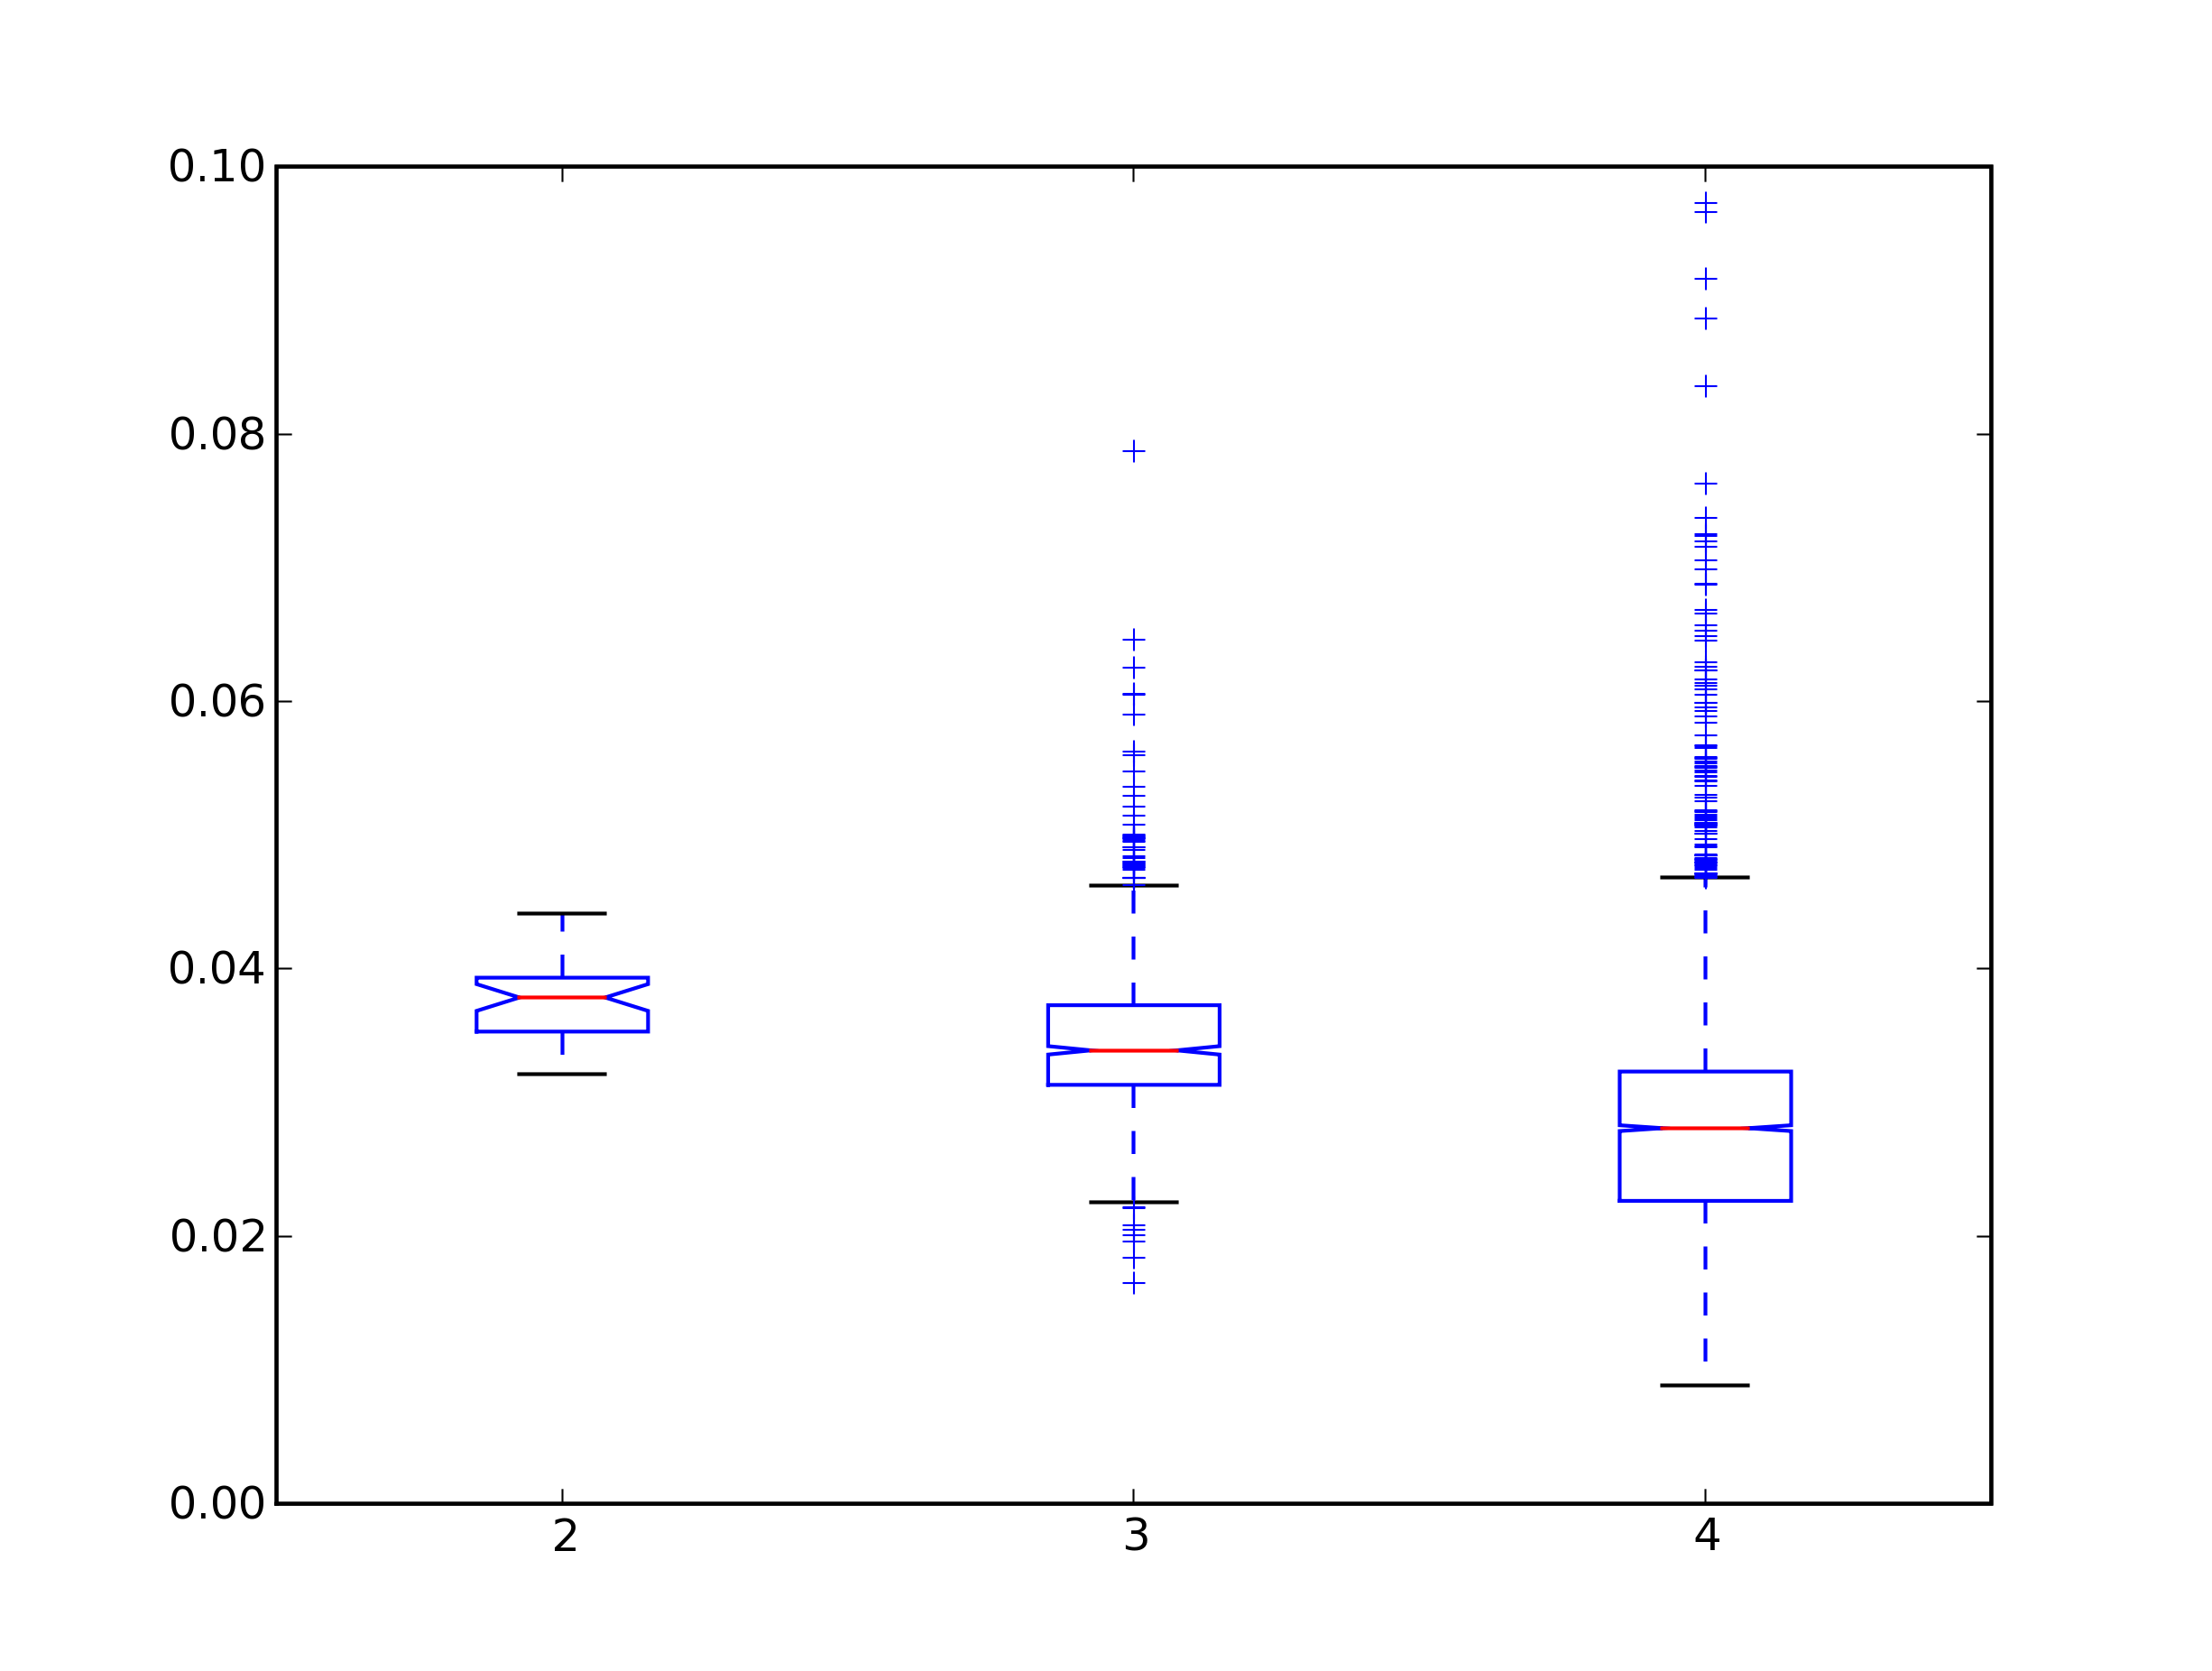
\includegraphics[width=\linewidth]{rook_iv_box.png}
\caption{This shows 3 box plots, each representing one group of neurons in a set
of SOMs trained with the same paremeters.}
\label{fRookIV}
\end{figure}

\begin{figure}
\centering
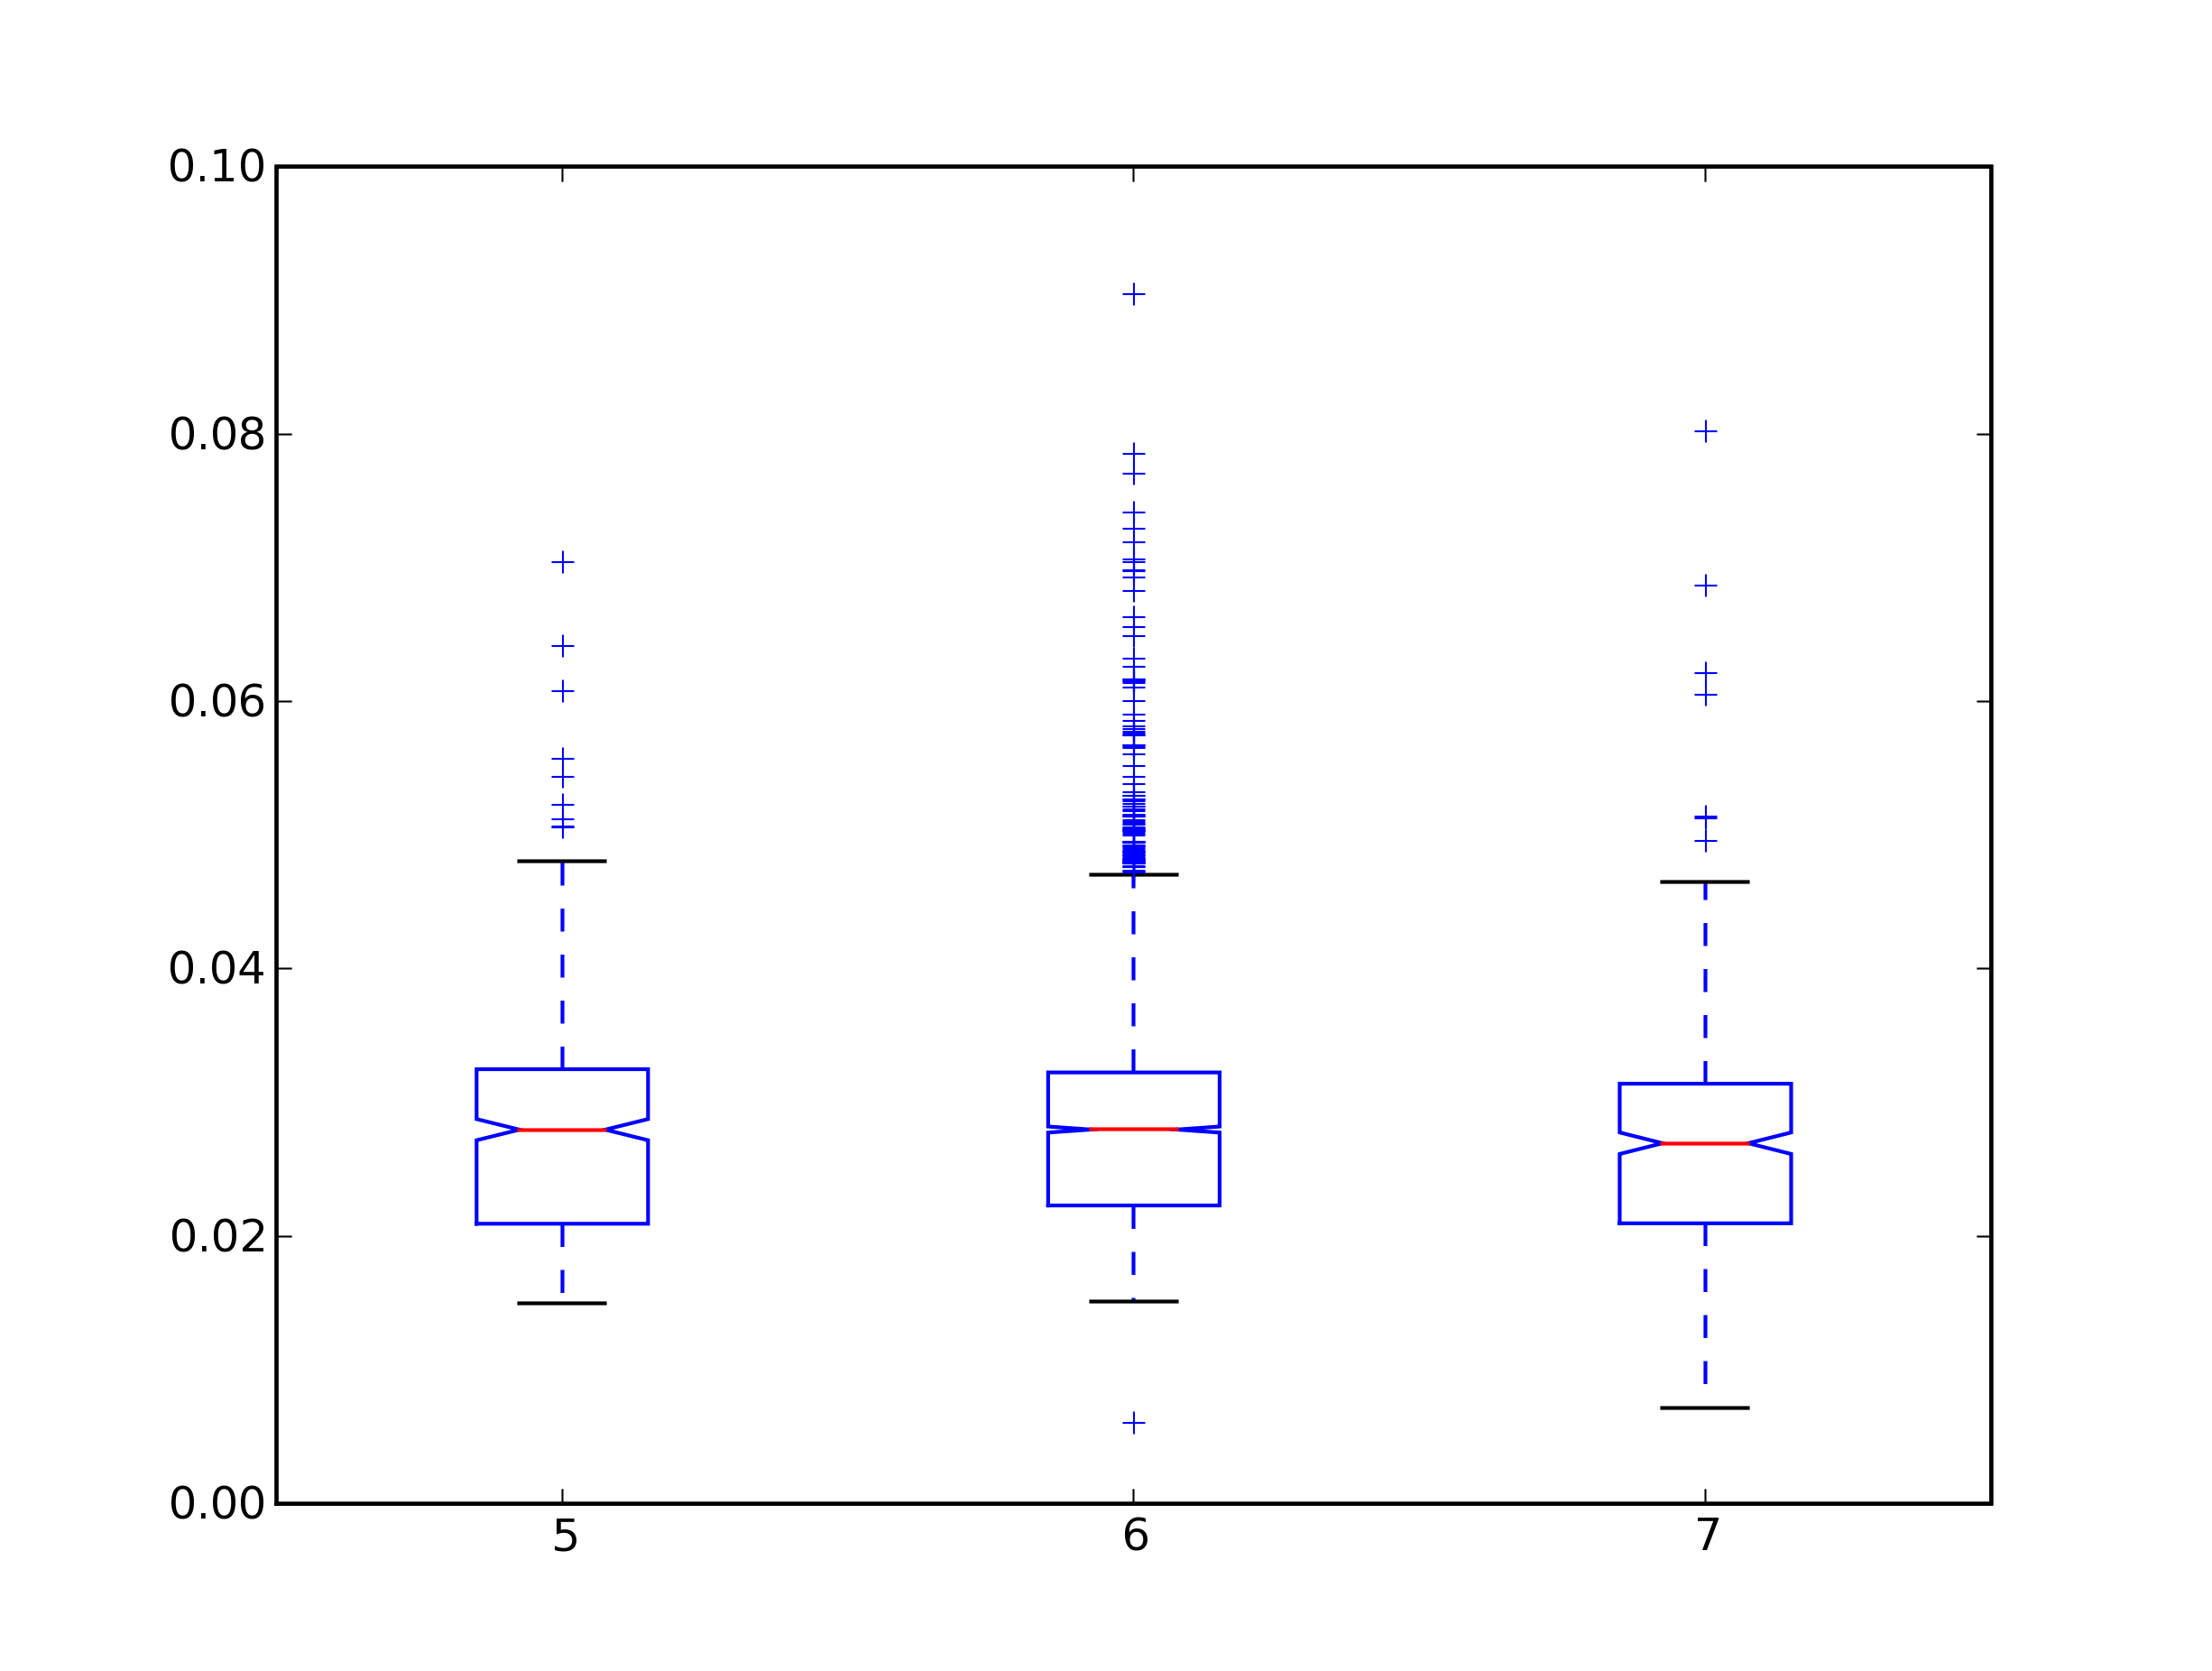
\includegraphics[width=\linewidth]{graph_iv_box.png}
\caption{This shows 3 box plots, each representing one group of neurons in a set
of SOMs trained with the same paremeters.}
\label{fGraphIV}
\end{figure}





To answer this question we need to setup a distance matrix (the distance of the
means) between each set of groups with in a given topology.  The table should
look like this...... 
\\
  2 3 4\\
2 0 + +\\
3 - 0 +\\
4 - - 0\\
\\
differance of means test\ldots
\ref{randomLabelTableRook}
\ref{randomLabelTableGraph}

\begin{table}
\caption{Random Labeling Mean Tests for rook case,  delta (p-Value)}
\label{randomLabelTableRook}
\begin{tabular}{|c||c|c|c|}
\hline
&2&3&4\\
\hline
\hline
2& & 0.012681 (0.009000)& 0.024790 (0.001000)\\
\hline
3& 0.012681 (0.011000)& & 0.012109 (0.001000)\\
\hline
4& 0.024790 (0.001000)& 0.012109 (0.001000)& \\
\hline
\end{tabular} \end{table}


\begin{table}
\caption{Random Labeling Mean Tests for graph case,  delta (p-Value)}
\label{randomLabelTableGraph}
\begin{tabular}{|c||c|c|c|}
\hline
&5&6&7\\
\hline
\hline
5& & 0.000362 (0.786000)& 0.001358 (0.480000)\\
\hline
6& 0.000362 (0.752000)& & 0.000996 (0.484000)\\
\hline
7& 0.001358 (0.503000)& 0.000996 (0.514000)& \\
\hline
\end{tabular} \end{table}




